\chapter{OSDOCR Filsofia}
\label{cap_osdocr_filosofia}

Neste capítulo é realizada uma reflexão sobre o problema e as consequentes propostas que são deste retiradas. Serão descritas decisões e modelos fundamentais da solução, assim como a arquitetura desta. 

\section{O problema}

Na sua essência, o problema abordado pode ser descrito como a aquisição de resultados não satisfatórios na aplicação de OCR sob documentos antigos com texto estruturado. 

Como se analisou no capítulo \ref{cap_estado_arte}, estes resultados podem ser melhorados através de múltiplas interações em múltiplas partes do processo do reconhecimento de texto: quer seja antes deste ser realizado, através de processamento de imagem; durante a deteção de texto, através da configuração proposta ao motor OCR; ou após através do tratamento dos resultados e do texto.

Estas diferentes interações são, na generalidade, aplicações sobre um input inicial de forma a transformá-lo, consequentemente resolvendo particularidades deste. Exemplos disto são: aplicação de técnicas de binarização que reduzem ruído ou imperfeições numa imagem; melhoria de resolução de uma imagem; correções ortográficas de texto; etc. Estas interações, podem então ser consideradas como um conjunto de ferramentas que podem ser aplicadas ao input do nosso problema de forma a abordar diferentes defeitos deste de acordo com as suas características; até porque, como também foi descrito para algumas destas, a sua utilização indiscriminada pode deteriorar, ao invés de melhorar, o produto final. As ferramentas comummente utilizadas não são explicitamente dedicadas ao problema de OCR em concreto, aumentando a sua utilidade e adaptabilidade para outras situações.
Tal reforça o intuito base do trabalho, da criação de um toolkit que proporcione um conjunto de funcionalidades independentes, com a intenção final de procurar melhorar os resultados da transcrição de texto.

Podemos então declarar aqui uma primeira proposta: 

\highlight{Proposta 1: A solução para o problema deve ser composta por um conjunto de ferramentas independentes, i.e. um toolkit.}[\normalsize]

Durante a análise do estado da arte, notou-se que para soluções para o problema de melhorar a aplicação de OCR, um processo com 3 partes principais pode ser identificado, sendo estas: pré-processamento de OCR, composto por processamento do input para realização de OCR, usualmente uma imagem; OCR, configurando o motor de OCR de acordo com as características do input, como a linguagem esperada do texto ou o dpi da imagem; pós-processamento de OCR, aplicando transformações nos resultados como, remover blocos de ruído, ordenar blocos identificados ou aplicar correções no texto. 

\begin{figure}[H]
     \centering
     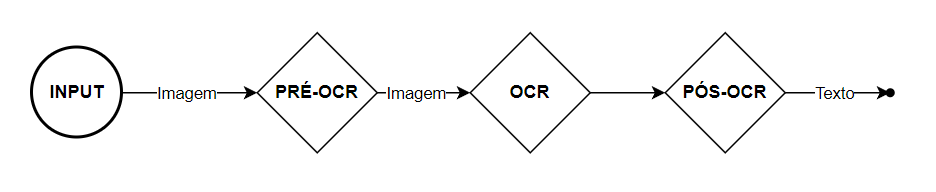
\includegraphics[width=1\textwidth]{images/diagramas/pipeline_alto_nivel.png}
     \caption{Aplicação de OCR com passos para melhoria de resultados}
     \label{fig:pipeline_high_level}
\end{figure}
 
Observando a figura \ref{fig:pipeline_high_level}, podemos identificar que a estrutura das soluções para aplicação de OCR é uma pipeline.

Estas pipelines podem ser elaboradas como uma sequência de aplicações das ferramentas acima mencionadas, como por exemplo:

\begin{figure}[H]
	\centering
	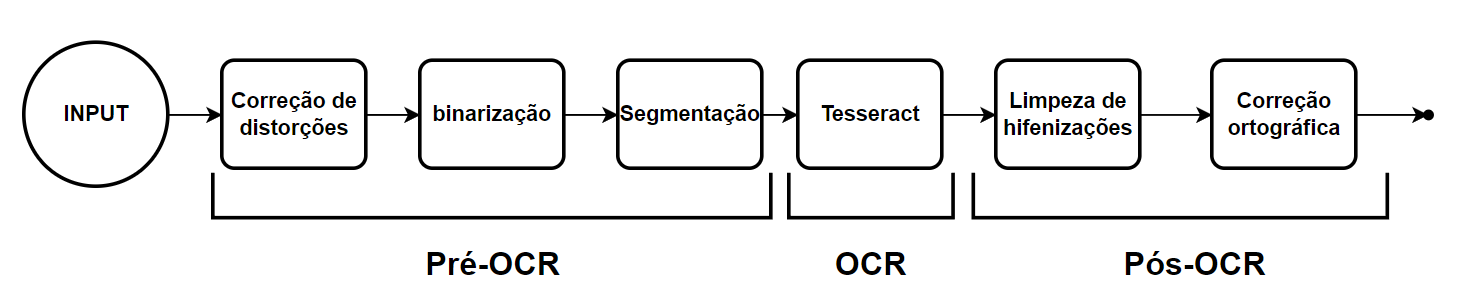
\includegraphics[width=1\textwidth]{images/diagramas/pipeline_exemplo.png}
	\caption{Exemplo de pipeline de aplicação de OCR}
	\label{fig:pipeline_example}
\end{figure}
 
 
Assumindo então a proposta da criação de um toolkit, e a necessidade de verificar a eficácia deste e criar casos de uso deste, torna-se claro que será útil o desenvolvimento de uma pipeline de aplicação de OCR, que faça uso do toolkit desenvolvido, assim como de outras ferramentas disponíveis e que abordem questões em falta no toolkit.

Seguindo o estudo realizado, esta pipeline será composta por 3 partes principais: pré-OCR, OCR e pós-OCR.


% proposta de pipeline

% proposta de pipeline composta por 3 areas principais, processamento de imagem, OCR, processamento de resultados


\highlight{Proposta 2: A solução para o problema deve possuir uma pipeline de aplicação de OCR que faça uso da toolkit desenvolvida.}[\normalsize]

\highlight{Proposta 3: A pipeline desenvolvida deve ser composta por 3 partes principais: pré-processamento de OCR, OCR e pós-processamento de OCR.}[\normalsize]
 
 
Como discutido, o uso de ferramentas independentes é interessante devido ao facto que diferentes inputs irão necessitar de tratamentos distintos de forma a obter os melhores resultados. Desta forma, é interessante que a pipeline desenvolvida não seja totalmente sequencial, de modo a aumentar a sua utilidade.



\begin{figure}[H]
	\centering
	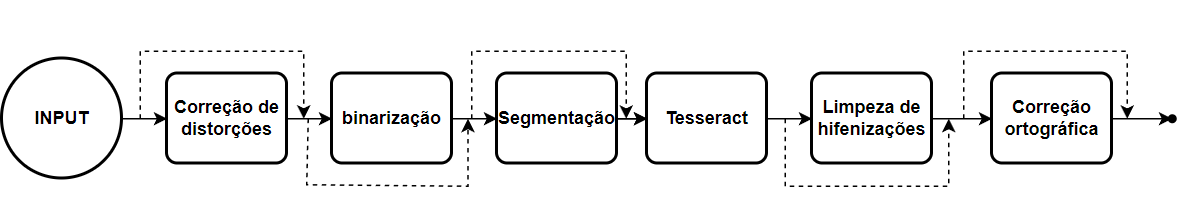
\includegraphics[width=1\textwidth]{images/diagramas/pipeline_exemplo_opcoes.png}
	\caption{Exemplo de pipeline de aplicação de OCR com blocos opcionais}
	\label{fig:pipeline_example_options}
\end{figure}

% proposta de pipeline composta por blocos opcionais

\highlight{Proposta 4: A pipeline deverá ser configurável. Permitirá, dentro dos blocos disponíveis, escolher aqueles que são aplicados.}[\normalsize]

Esta pipeline, seguindo a estrutura explicada de aplicação de OCR, apresentará 3 partes principais onde, a primeira - pré-OCR - irá lidar com um input do tipo imagem e terá como output uma imagem; a segunda - OCR - terá como input uma imagem e devolverá os resultados de OCR; e a última - pós-OCR - irá ter como input os resultados de OCR, e terá como output a transcrição do texto da imagem.

Nota-se uma ambiguidade no output da 2º parte e no input da 3º, os resultados de OCR. Tal, deve-se ao facto de motores OCR, como o Tesseract, permitirem vários tipos de output. É então relevante a criação de um estrutura de dados universal para a representação de resultados OCR.

Como estudado no capítulo \ref{cap_estado_arte}, tais representações já possuem um standard um formato de ficheiro, como \textbf{HOCR}, portanto a estrutura de dados escolhida deve ser baseado nestes, ou ser convertível para o standard.

% proposta de estrutura de dados unica para a represantacao de resultados OCR

\highlight{Proposta 5: Criação de uma estrutura de dados universal para a representação dos resultados de OCR.}[\normalsize]

\highlight{Proposta 6: A estrutura de dados universal para a representação dos resultados de OCR deve ser baseada ou convertível num formato standard.}[\normalsize]


No estudo do estado da arte, foi possível compreender que a criação de algoritmos ubíquos para todos os tipos de documentos é um empreendimento com diminutas chances de sucesso, sendo que para muitos problemas, como por exemplo o cálculo da ordem de leitura, mesmo focando num só tipo de documento como jornais, os resultados podem não ser satisfatórios devido à diversidade de estruturas existentes. Consequentemente, é esperado que a pipeline não seja sempre suficiente na resolução do problema. 
Deste modo, servindo também como outro caso de uso do toolkit, a criação de uma ferramenta que permite ao utilizador um maior manuseamento dos resultados de OCR é uma proposta para a solução. 

Tendo em conta a forte qualidade visual desta área de trabalho, onde se procura processar e analisar imagens de documentos, a utilidade e usabilidade desta ferramenta de edição é elevada ao definirmos que o editor seja gráfico.

% proposta de editor de estrutura de dados para realizacao de afinações manuais

\highlight{Proposta 7: A solução do problema deverá possuir um editor gráfico dos resultados de OCR, que permita aplicar ferramentas propostas pelo toolkit.}[\normalsize]


% apanhado das proposta

Em suma, as propostas definidas para o desenho da solução são:

\begin{enumerate}[label=\textbf{\arabic*}]\setlength\itemsep{-0.8em}
	\item A solução para o problema deve ser composta por um conjunto de ferramentas independentes, i.e. um toolkit.
	\item A solução para o problema deve possuir uma pipeline de aplicação de OCR que faça uso da toolkit desenvolvida.
	\item A pipeline desenvolvida deve ser composta por 3 partes principais: pré-processamento de OCR, OCR e pós-processamento de OCR.
	\item A pipeline deverá ser configurável. Permitirá, dentro dos blocos disponíveis, escolher aqueles que são aplicados.
	\item Criação de uma estrutura de dados universal para a representação dos resultados de OCR.
	\item A estrutura de dados universal para a representação dos resultados de OCR deve ser baseada ou convertível num formato standard.
	\item A solução do problema deverá possuir um editor gráfico dos resultados de OCR, que permita aplicar ferramentas propostas pelo toolkit.
\end{enumerate}


\section{Modelos}

Realizada uma acessão mais concreta do problema e das soluções que para este são sugeridas, segue-se uma discussão sobre os elementos fundamentais que servirão como base do trabalho a realizar. No caso deste problema, os de maior relevância são os tipos de dados que serão processados: imagens para processamento e realização de OCR; e estruturas de dados para representação dos resultados OCR.

\subsection{Imagem}

A área de computação de visão é extensa e complexa, apresentando já a sua medida de standards e ferramentas disponíveis. Neste sentido, no propósito deste problema, apenas sobra escolher o tipo de estruturas de dados que se pretende usar de forma a gerar uma consistência no projeto.

Sendo que a componente prática do projeto será maioritariamente produzida utilizando Python, optou-se pela utilização das estruturas de dados oferecidas pelo \textbf{open-cv} devido à compreensiva biblioteca de métodos disponíveis, utilidade para o problema e reputação na área.

\subsection{OCR Tree - estrutura de dados para resultados OCR}

Os resultados de OCR podem tomar múltiplas formas; tomando como exemplo a utilização de Tesseract, este permite a geração de output diretamente no formato de texto, dicionário, pdf, hocr, etc.. Deste modo, é necessário decidir o tipo de formato que se pretende para ser trabalhado pelas ferramentas da solução.

Tendo em conta os tipos de problemas que se pretendem resolver - remover ruído detetado como texto, calcular ordem de leitura, categorizar elementos detetados -, é necessária informação além do texto detetado, sendo útil informações geométricas sobre este ex.: posição na imagem, dimensões de elementos detetados. Deste modo, é útil observar o standard HOCR.

\begin{figure}[H]
	\centering
	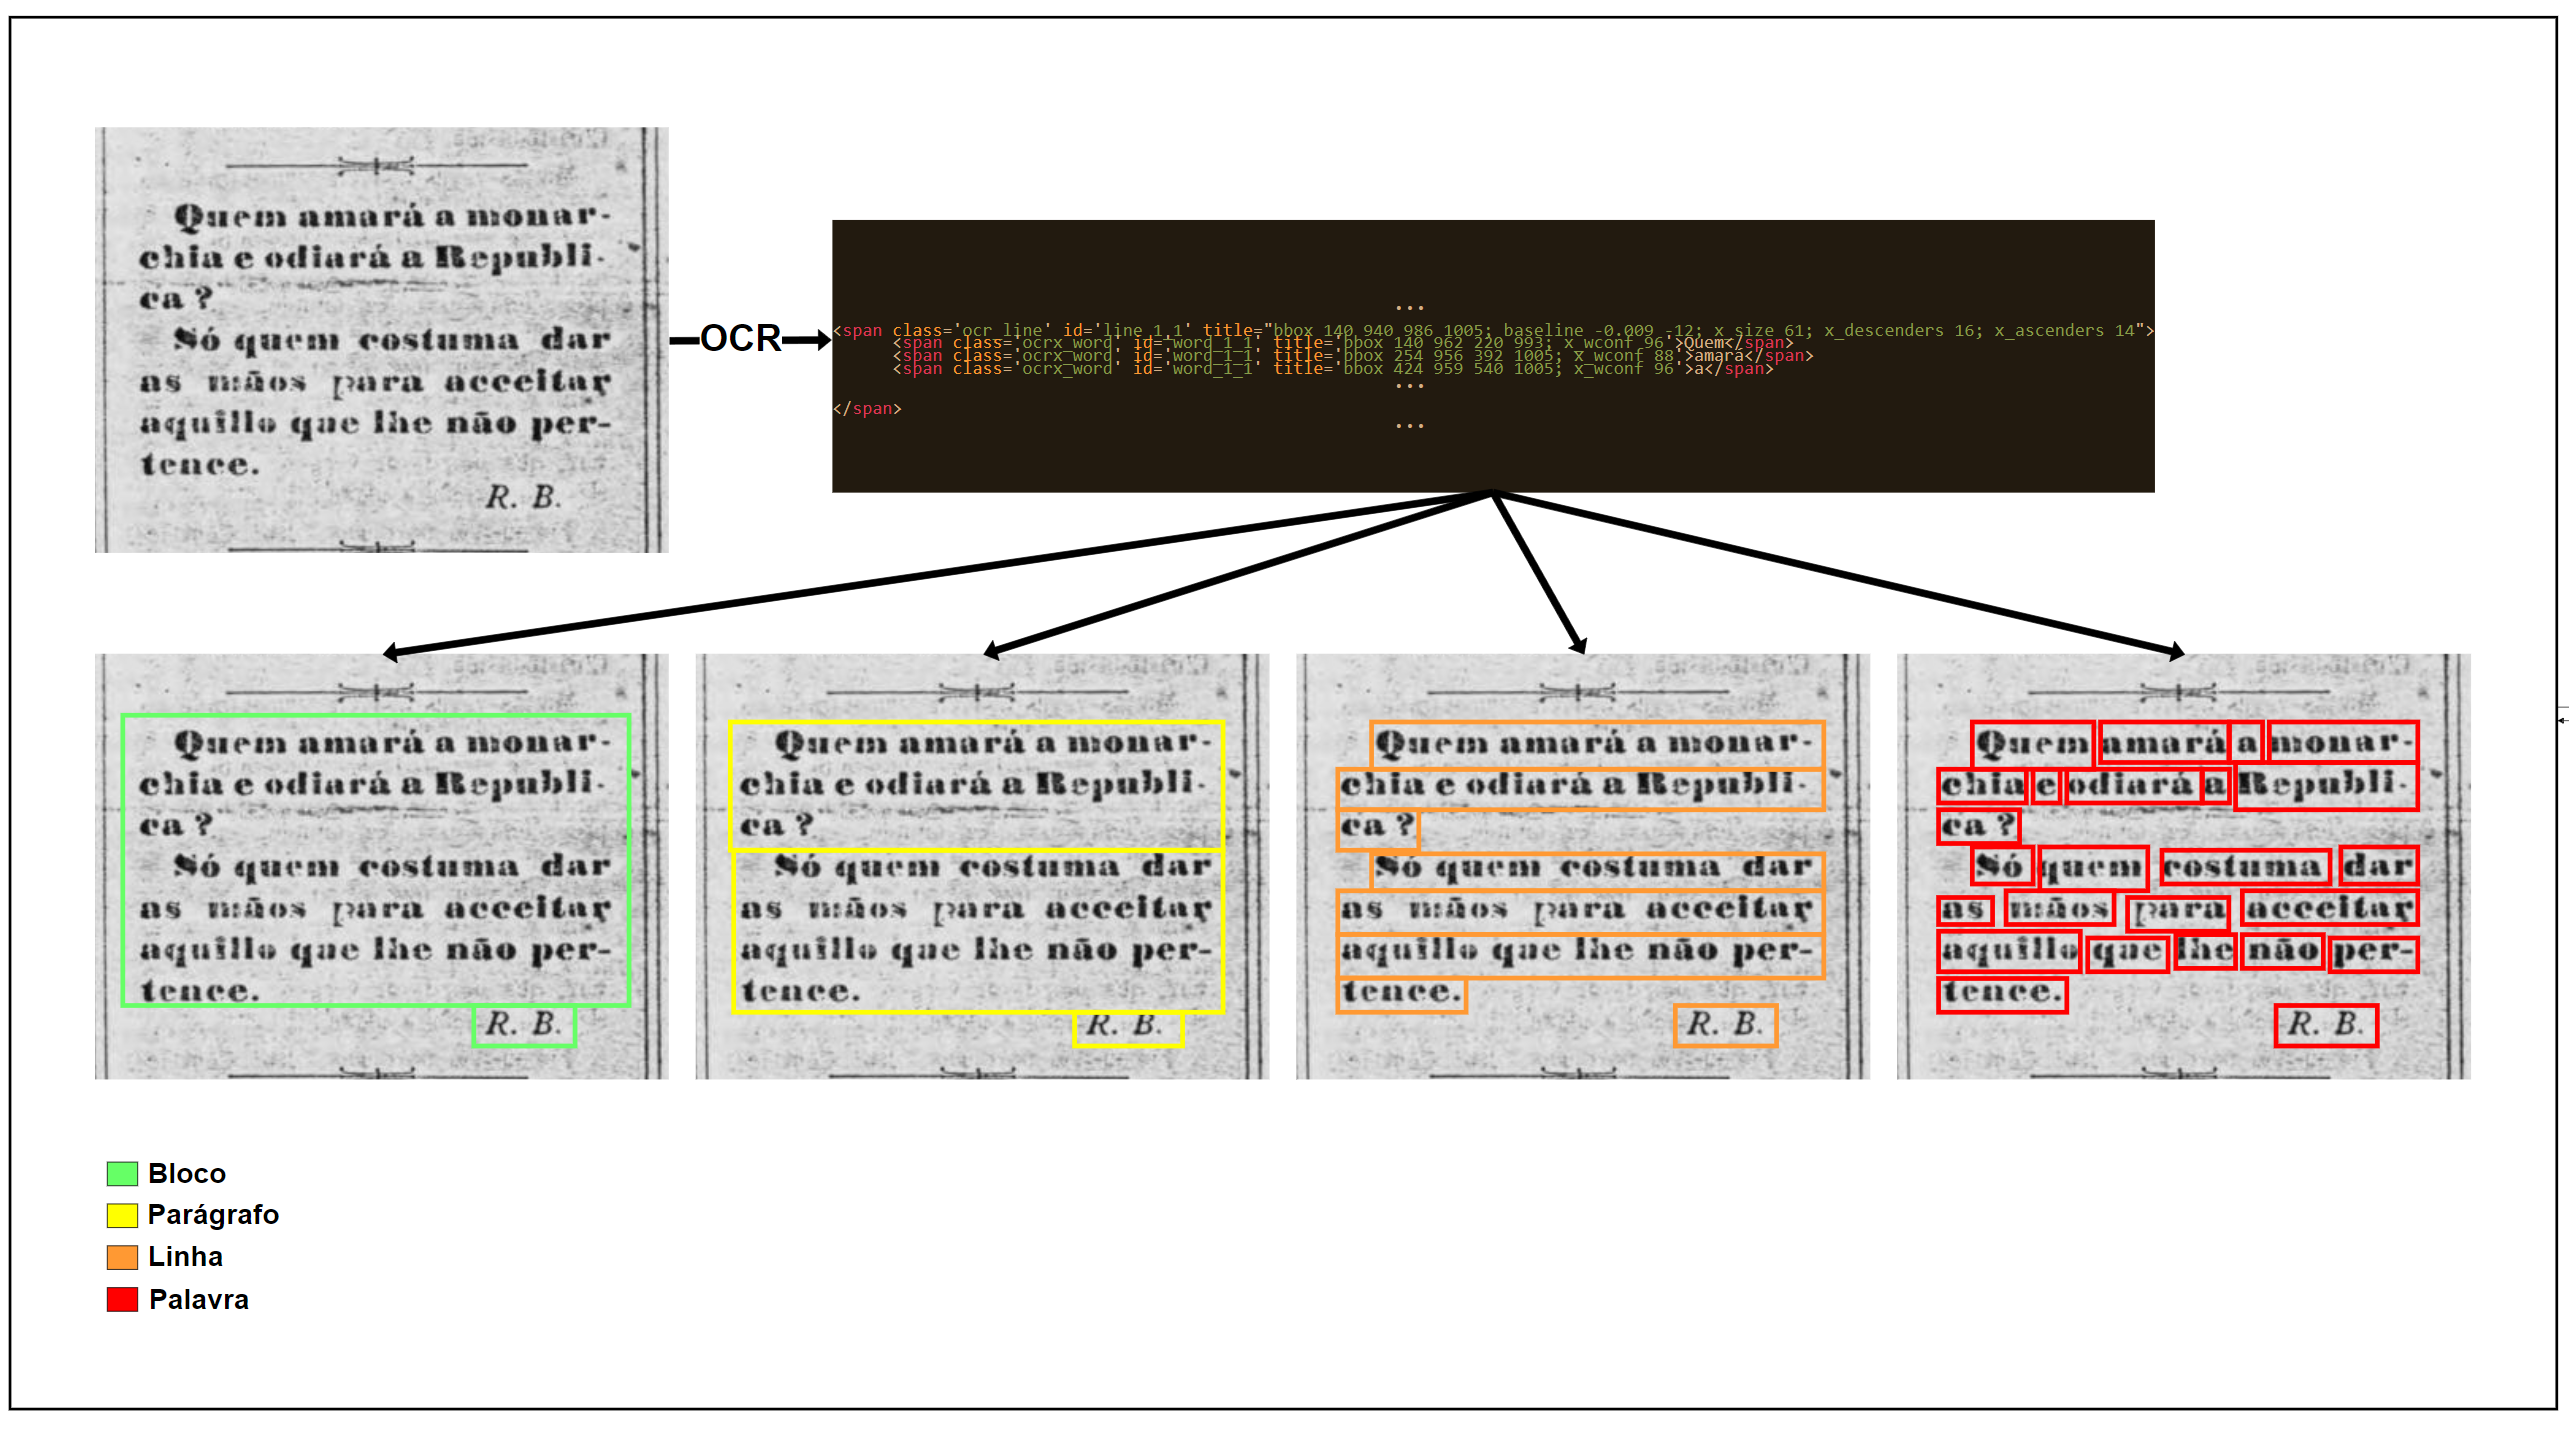
\includegraphics[width=1\textwidth]{images/ilustracoes/hocr_visual_representation.png}
	\caption{Representação visual dos resultados de OCR armazenados em formato HOCR}
	\label{fig:hocr_visual_representation}
\end{figure}


Como podemos observar na figura \ref{fig:hocr_visual_representation}, é possível criar uma representação visual dos resultados de OCR a partir de ficheiros HOCR, mais digerível do que o seu formato base. Este tipo de representação disponibiliza uma importante ferramenta de debugging de métodos que transformem os resultados OCR, assim como uma melhor compreensão sobre a natureza dos resultados OCR como uma estrutura de dados do tipo árvore. Esta representação visual é apenas possível devido à informação extra armazenada sobre o texto reconhecido, como as bounding boxes.

A partir deste tipo de ficheiro, temos então que a informação mais relevante que podemos obter é:

\begin{itemize}\setlength\itemsep{-0.8em}
	\item posição e dimensões do texto detetado, através do armazenamento de bounding boxes.
	\item diferentes níveis de deteção de texto, permitindo uma estruturação base deste.
		\begin{itemize}\setlength\itemsep{-0.8em}
			\item pagina
			\item bloco
			\item parágrafo
			\item linha
			\item palavra
		\end{itemize}
	\item identificadores dos elementos.
	\item nível de confiança do texto detetado.
\end{itemize}

No propósito da criação de uma classe de dados para o papel da estrutura de dados universal para representar os resultados OCR, seguiu-se com um desenho baseado numa árvore, denominada \textbf{OCR Tree}, e que irá possuir, como atributos base, os acima listados.

Esta classe irá, para cumprir standards, possuir um conversor de e/para HOCR. 

Maior detalhe sobre esta está disponível nos capítulos seguintes, dedicados à implementação da solução.


\section{Arquitetura da solução}

Descritas as decisões fundamentais sobre a solução e os modelos base que a irão compor, expõe-se nesta secção a arquitetura desta, na sua generalidade e das suas partes.

A arquitetura geral da solução é composta por 3 componentes principais, correspondentes às propostas anteriores: o "OSDOCR Toolkit", que será um conjunto de ferramentas desenvolvidas para melhorar os resultados de OCR; a "OSDOCR Pipeline" que será uma aplicação do toolkit, assim como de algumas soluções já existentes, no formato de uma pipeline versátil; "OSDOCR Editor" que será uma segunda aplicação do toolkit, com o intuito de permitir um manuseamento mais delicado dos resultados OCR.

\begin{figure}[H]
	\centering
	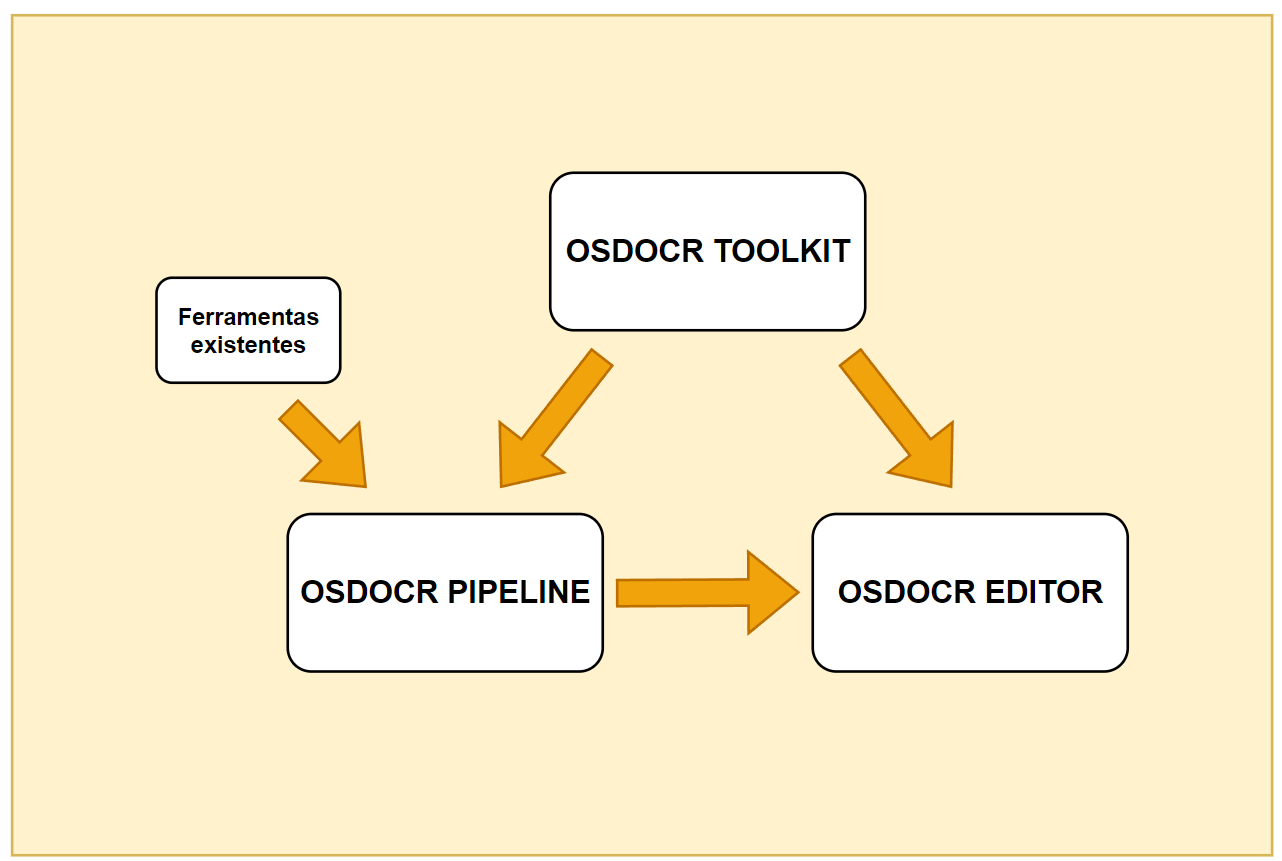
\includegraphics[width=1\textwidth]{images/diagramas/arquitetura_geral.png}
	\caption{Arquitetura geral da solução}
	\label{fig:arquitetura_geral}
\end{figure}

A maioria do código desenvolvido foi utilizando \textbf{Python}, com algumas instâncias de \textbf{C}.

\subsection{OSDOCR Toolkit}


A componente de OSDOCR Toolkit servirá como base para as outras duas componentes da solução e, como o nome desta indica, servirá como o produto principal a ser importado para projetos futuros.

Esta é composta por 3 módulos fundamentais, cada um dedicado a uma dada área: "Imagem", disponibilizando ferramentas de processamento e análise de imagens de documentos; "OCR Tree", com ferramentas que permitem manipulação de resultados OCR representados pela classe OCR Tree; "Texto", para o processamento de texto e geração de output textual.

\begin{figure}[H]
	\centering
	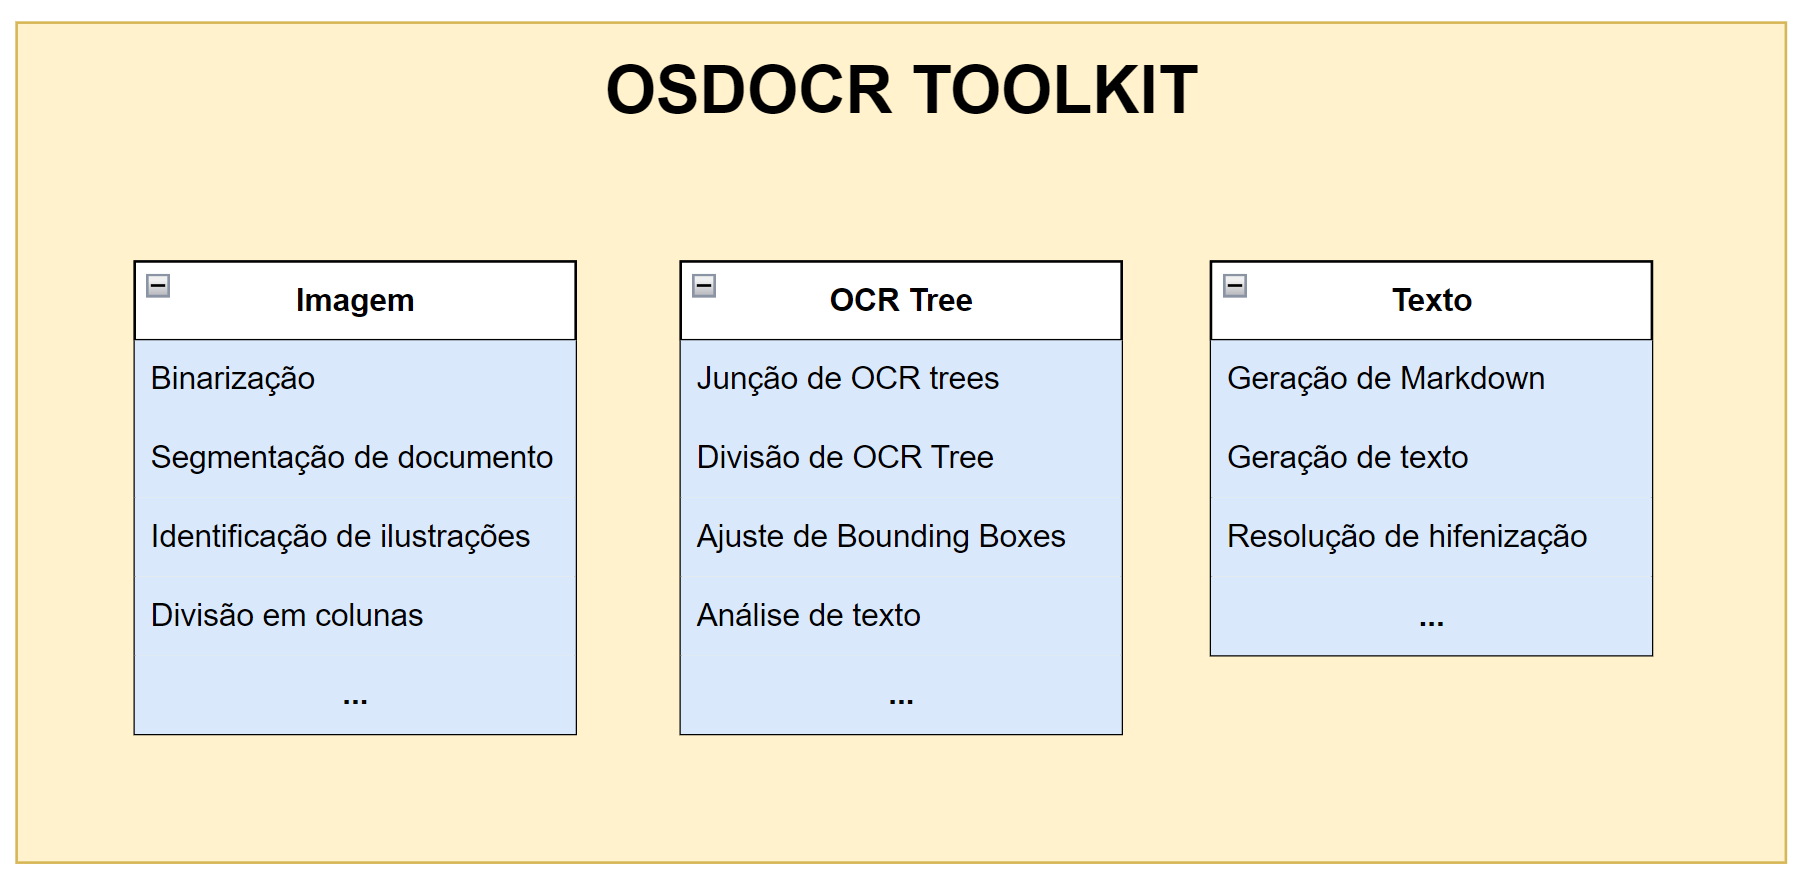
\includegraphics[width=1\textwidth]{images/diagramas/arquitetura_toolkit.png}
	\caption{Arquitetura OSDOCR Toolkit}
	\label{fig:arquitetura_toolkit}
\end{figure}


\subsection{OSDOCR Pipeline}

A componente de OSDOCR Pipeline é um exemplo de uma aplicação do toolkit criado no caso de uso clássico para a aplicação de OCR. Este apresenta portanto os 3 procedimentos principais deste uso clássico: pré-processamento OCR, tratamento e análise da imagem de input; OCR; pós-processamento OCR, tratamento e interpretação dos resultados.

Como proposto, esta componente torna-se mais útil se tiver um maior nível de versatilidade. Deste modo, mesmo os procedimentos gerais de pré e pós processamento são opcionais, como se pode ver na figura \ref{fig:arquitetura_pipeline_high_level}.

\begin{figure}[H]
	\centering
	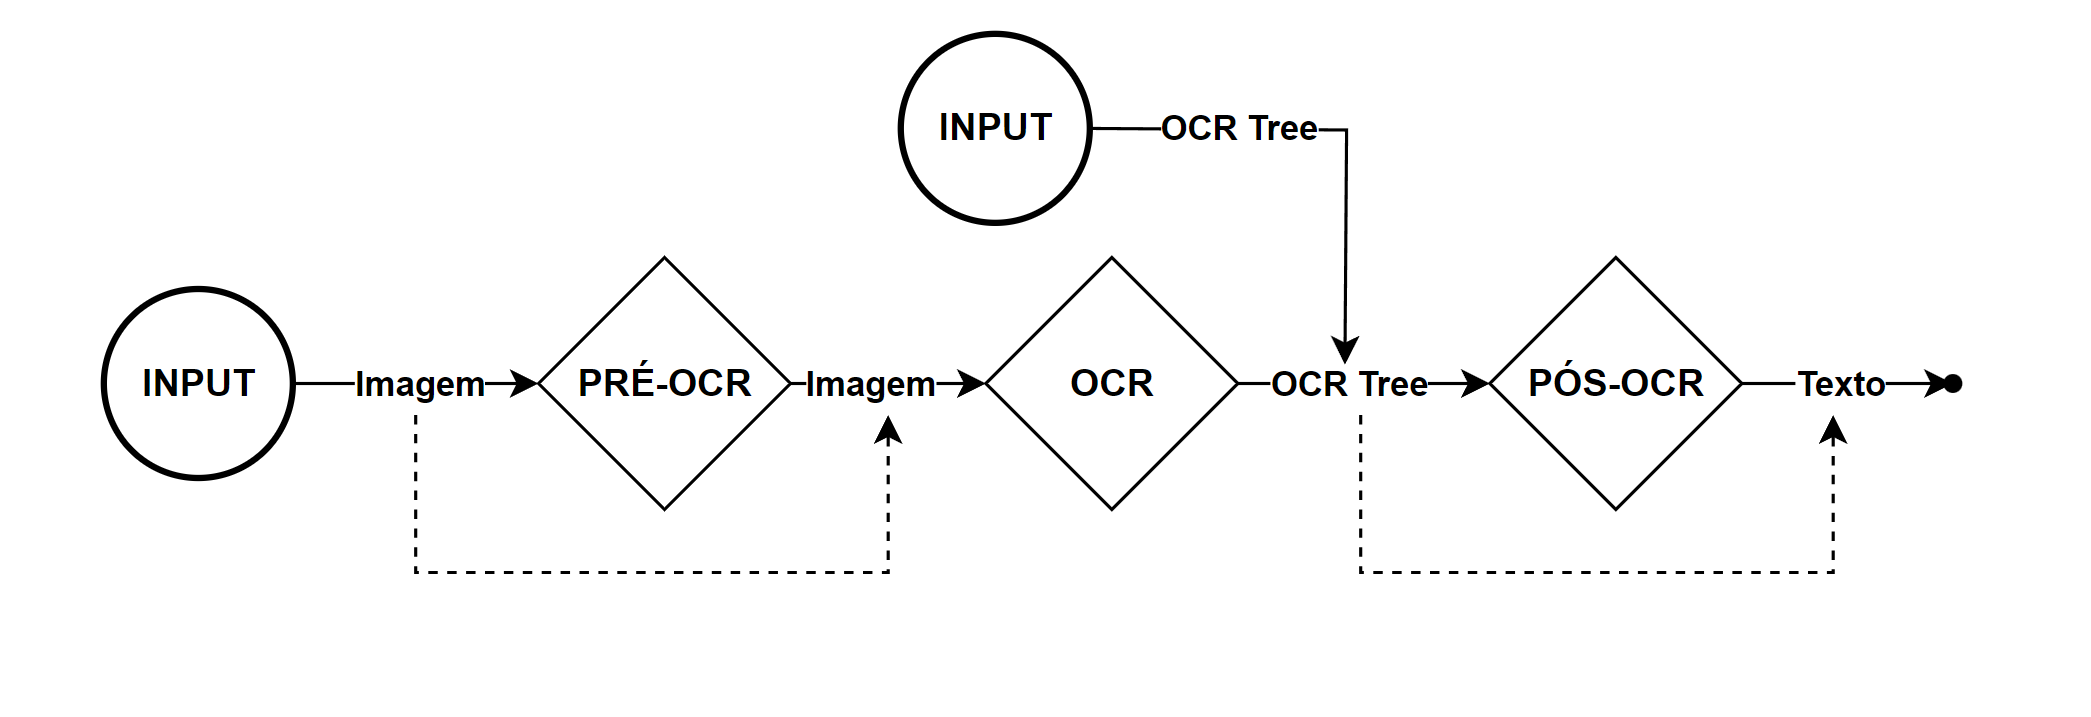
\includegraphics[width=1\textwidth]{images/diagramas/arquitetura_pipeline_high_level.png}
	\caption{Arquitetura OSDOCR Pipeline - high level}
	\label{fig:arquitetura_pipeline_high_level}
\end{figure}

Como também se pode verificar na figura, os tipos de dados manipulados na pipeline são contidos - havendo apenas 3 tipos usados -, auxiliando a possibilidade de a configurar.


Cada um dos procedimentos é composto por blocos elementares, que, mantendo a mesma lógica de versatilidade, são opcionais.


\begin{figure}[H]
	\centering
	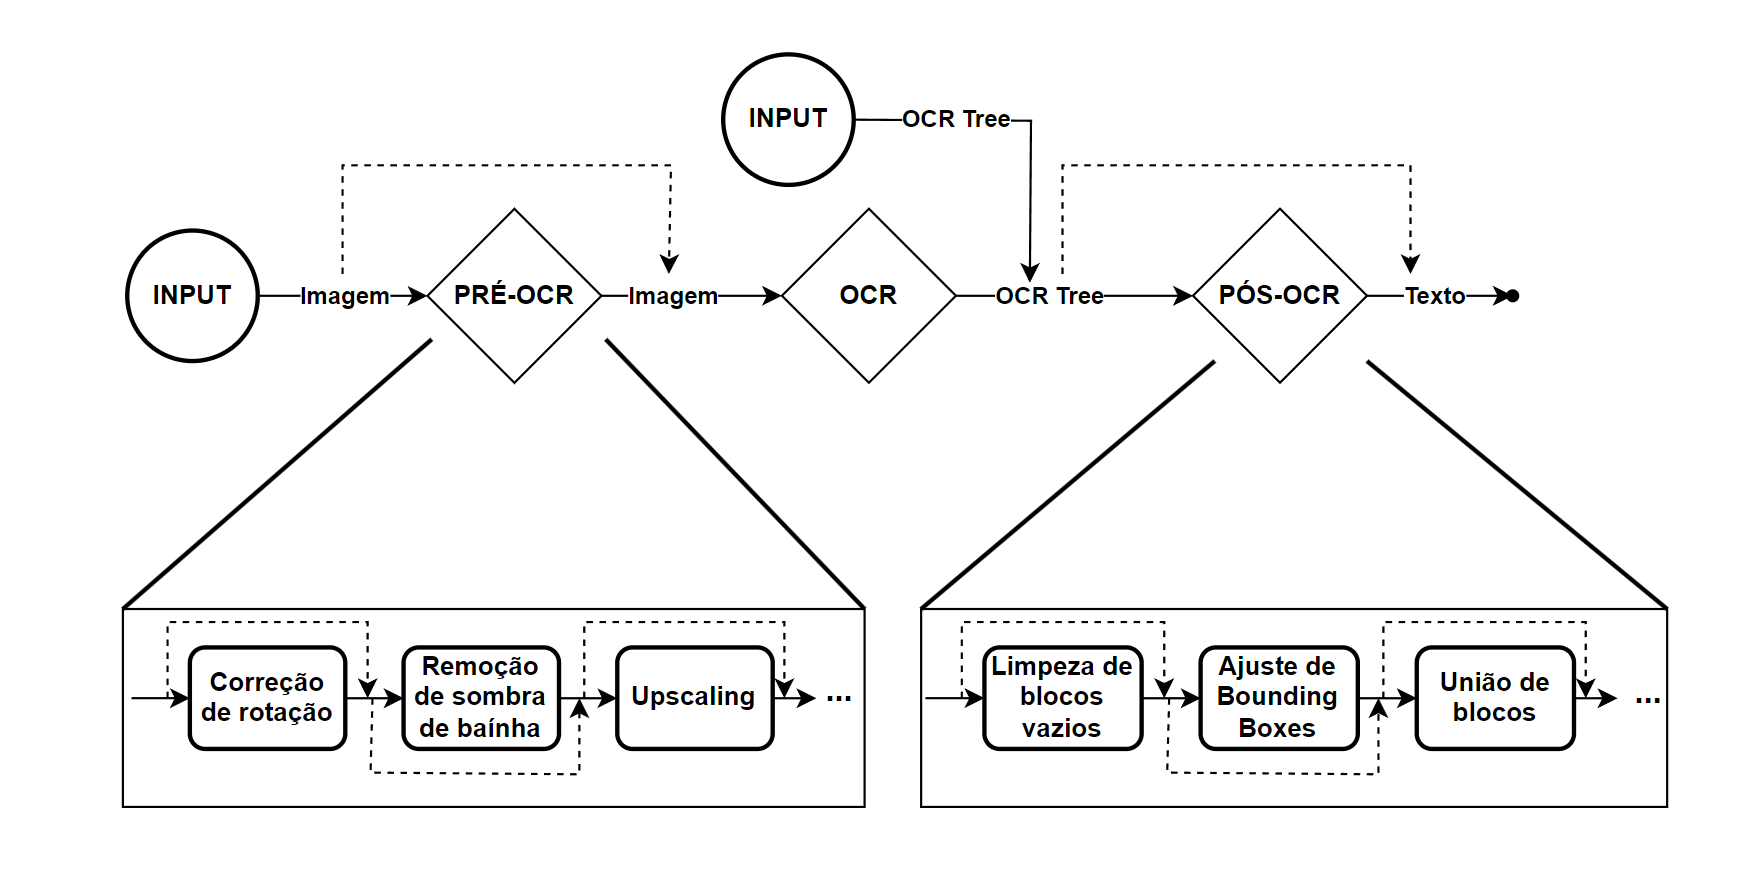
\includegraphics[width=1\textwidth]{images/diagramas/arquitetura_pipeline_reduced.png}
	\caption{Arquitetura OSDOCR Pipeline - reduzida}
	\label{fig:arquitetura_pipeline_reduced}
\end{figure}

Alguns destes blocos, principalmente no que toca a manipulação de imagem, fazem uso de soluções externas disponíveis, ex.: upscaling de imagem utilizando modelos de Deep Learning open-source.

Maior detalhe sobre estes blocos será discutido no capítulo de implementação da pipeline.


\subsection{OSDOCR Editor}

O OSDOCR Editor é um GUI relativamente simples, sendo que apresenta uma proposta bastante focada, a de manipulação de OCR Tree. 

Este segue uma arquitetura \textbf{MVC} (Model View Controller), tendo sido desenvolvido a \textbf{View} geral utilizando a biblioteca \textbf{PySimpleGui}. Para complemento desta, e devido à permitida compatibilidade, foi utilizado \textbf{MatplotLib} no desenvolvimento do canvas visualizador e de manipulação da OCR Tree.

\begin{figure}[H]
	\centering
	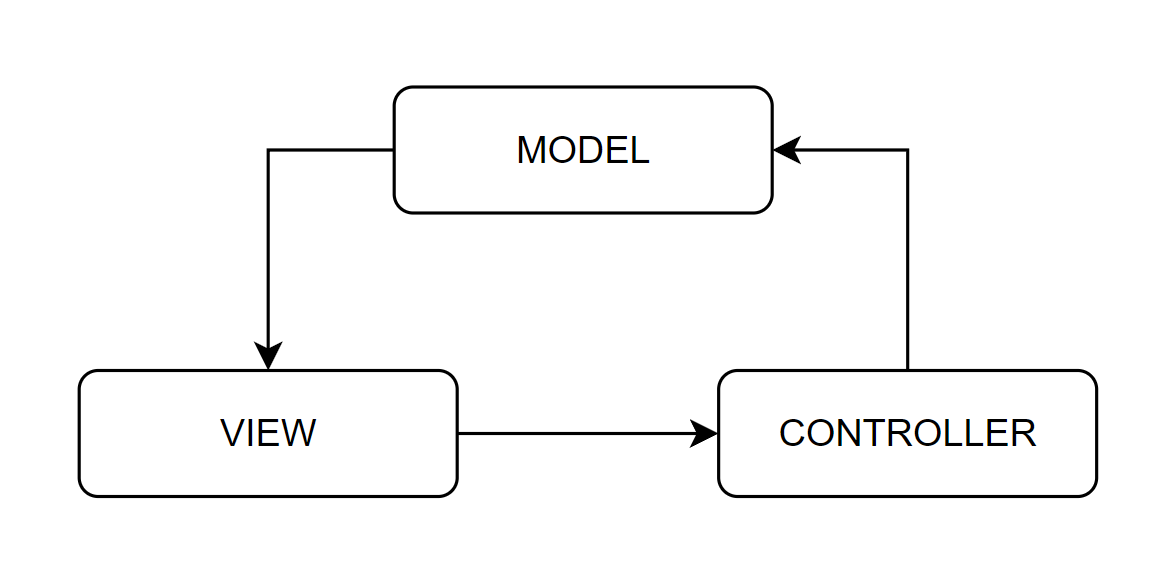
\includegraphics[width=1\textwidth]{images/diagramas/MVC.png}
	\caption{Arquitetura MVC}
	\label{fig:arquitetura_mvc}
\end{figure}

O \textbf{controlador} neste GUI provêm - para além do MatplotLib e do PySimpleGui - das ferramentas disponibilizadas pelo OSDOCR Toolkit e, nalguns casos como por exemplo de aplicação de OCR numa área focada de uma imagem, da OSDOCR Pipeline.

Os constituintes principais do \textbf{modelo} são: imagem de input; OCR Tree; abstrações de OCR Tree, ex.: artigos (lista de listas OCR Tree).








